\documentclass[12pt, xcolor=dvipsnames,svgnames,x11names]{article}
\usepackage{xcolor}
\usepackage{amsmath}
%\usepackage{universityos}
\usepackage{xspace}
\usepackage{url}
\usepackage[colorlinks=true,bookmarks=false,linkcolor=black,urlcolor=blue,citecolor=black]{hyperref}
\usepackage{minted}
\usepackage{fancyhdr}
\usepackage[top=1in,bottom=1in,left=1in,right=1in]{geometry}
\usepackage{multicol}
\usepackage{pgfplots}
\usetikzlibrary{circuits.logic.US}
% \usepackage{tgschola}
\let\temp\rmdefault
\usepackage{mathpazo}
\let\rmdefault\temp

\definecolor{roseRed}{HTML}{e20047}
\definecolor{coolGray}{HTML}{474747} % Neutral gray to contrast roseRed
\definecolor{mocha}{HTML}{a47864}
\definecolor{sage}{HTML}{8a9a5b}
\definecolor{dustyblue}{HTML}{6e8ca0}
\definecolor{terracotta}{HTML}{c87f5b}
\definecolor{lavender}{HTML}{9d8bb0}
\definecolor{darkmocha}{HTML}{7a5a4b}
\definecolor{darksage}{HTML}{667244}
\definecolor{darkdustyblue}{HTML}{526878}
\definecolor{darkterracotta}{HTML}{9e6347}
\definecolor{darklavender}{HTML}{766688}
\definecolor{winery}{HTML}{7e212a}

\definecolor{lightmocha}{HTML}{c2a190}
\definecolor{lightmocha1}{HTML}{d1b09c}
\definecolor{lightmocha2}{HTML}{e2c4b0}
\definecolor{lightmocha3}{HTML}{f0d9c7}

\definecolor{androidBlue}{HTML}{8AB4F8}
\definecolor{androidBlueLight}{HTML}{E8F0FE}
\definecolor{androidGreen}{HTML}{81C995}
\definecolor{androidGreenLight}{HTML}{E6F4EA}

% Red variants - based on Android's "error" and warning colors
\definecolor{androidRed}{HTML}{F28B82}
\definecolor{androidRedLight}{HTML}{FADAD7}

% Yellow variants - based on Android's accent/warning colors
\definecolor{androidYellow}{HTML}{FDD663}
\definecolor{androidYellowLight}{HTML}{FEF7E0}

% Purple variants - based on Android's system UI accents
\definecolor{androidPurple}{HTML}{D7AEFB}
\definecolor{androidPurpleLight}{HTML}{F4EAFC}

% Orange variants - based on Android's notification colors
\definecolor{androidOrange}{HTML}{FCAD70}
\definecolor{androidOrangeLight}{HTML}{FEEADC}

% Teal variants - based on Android's Material You palette
\definecolor{androidTeal}{HTML}{78D9EC}
\definecolor{androidTealLight}{HTML}{E6F6F9}

% Gray variants - based on Android's neutral colors
\definecolor{androidGray}{HTML}{DADCE0}
\definecolor{androidGrayLight}{HTML}{F1F3F4}

\usepackage{biolinum} % included with the {Libertine} font package
\renewcommand{\familydefault}{\sfdefault}



\usepackage[many]{tcolorbox}
\usepackage{CJKutf8}

\newcommand{\hw}{Classwork 06: Discrete Difference, Operations on Signals}
\newcommand{\duedate}{September 14, 2026}


% Redefine \maketitle to include tcolorbox
\makeatletter
\renewcommand{\maketitle}{%
    \begin{center}
        \begin{tcolorbox}[
            enhanced,
            colback=white,
            colframe=red!70!black,
            arc=0mm,
            title={\textcolor{white}{\bfseries CPE 381 \@title}},
            coltitle=white,
            fonttitle=\bfseries\large,
            attach boxed title to top left={xshift=10pt, yshift=-\tcboxedtitleheight/2},
            boxed title style={
            sharp corners,
            colback=red!70!black,
            frame hidden,
            boxrule=0pt,
            left=10pt, right=10pt,
            top=3pt, bottom=3pt
            }
        ]
        \large
        \vspace{10pt}
        \noindent Student Name (as in Canvas): \underline{\hspace{8cm}} 
        
        \vspace{10pt}
        \noindent A Number: \underline{\hspace{12cm}}

        \vspace{10pt}
        \noindent Points: 20 \quad Duration: 15 minutes \hfill \quad Due:~\duedate  ~(In-Class)

            \end{tcolorbox}
    \end{center}
}
\makeatother

\setlength{\parindent}{0pt}
\setlength{\parskip}{4pt}%

\usepackage{tikz}
\usepackage{pgfplots}

\newcommand{\coursenumber}{CPE381}
\newcommand{\courseyear}{2026\xspace}
\newcommand{\coursedatetime}{Mon/Wed 11:20 AM -- 12:40 PM\xspace}
\newcommand{\coursetitle}{Signals and Systems for Computer Engineers\xspace}
\newcommand{\courseterm}{Fall, \courseyear}
\newcommand{\courseurl}{\url{http://uah.instructure.com/}}
\newcommand{\courselocation}{ENG 207\xspace}
\newcommand{\courselocationurl}{TBD}

\newcommand{\instructorname}{Rahul Bhadani\xspace}
\newcommand{\instructoremail}{\href{mailto:rahul.bhadani@uah.edu}{rahul.bhadani@uah.edu}}
\newcommand{\instructoroffice}{ENG 217-H\xspace}
\newcommand{\instructorofficehours}{Mon/Tue/Wed 2:00 PM - 4:00 PM}


% \everymath{\color{Navy}}
\everydisplay{\color{roseRed}}
\usepackage{sectsty}
\sectionfont{\color{dustyblue}}  % sets colour of sections
\subsectionfont{\color{terracotta}}  % sets colour of sections
\subsubsectionfont{\color{lavender}}  % sets colour of sections


\def\m@th{\normalcolor\mathsurround\z@}

\setlength{\parskip}{\baselineskip}%
\setlength{\parindent}{0pt}%

%%%%%%%%%%%%%%%%%%%%%%%%%%%%%%%%%%%%%%%%%%%%%%%%%%%%%%%%%%%%%%%%%%%%%


\def\e{{\textrm{e}}}
\def\d{\textrm{d}}
\def\T{{\textsf{T}}}
\def\sech{{\textrm{sech}}}
\def\x{{\mathbf x}}

\def\++{{$^{++}$}}

\def\Abb{{\mathbb A}}
\def\Bbb{{\mathbb B}}
\def\Cbb{{\mathbb C}}
\def\Dbb{{\mathbb D}}
\def\Ebb{{\mathbb E}}
\def\Fbb{{\mathbb F}}
\def\Gbb{{\mathbb G}}
\def\Hbb{{\mathbb H}}
\def\Ibb{{\mathbb I}}
\def\Jbb{{\mathbb J}}
\def\Kbb{{\mathbb K}}
\def\Lbb{{\mathbb L}}
\def\Mbb{{\mathbb M}}
\def\Nbb{{\mathbb N}}
\def\Obb{{\mathbb O}}
\def\Pbb{{\mathbb P}}
\def\Qbb{{\mathbb Q}}
\def\Rbb{{\mathbb R}}
\def\Sbb{{\mathbb S}}
\def\Tbb{{\mathbb T}}
\def\Ubb{{\mathbb U}}
\def\Vbb{{\mathbb V}}
\def\Wbb{{\mathbb W}}
\def\Xbb{{\mathbb X}}
\def\Ybb{{\mathbb Y}}
\def\Zbb{{\mathbb Z}}



\def\Acal{{\mathcal A}}
\def\Bcal{{\mathcal B}}
\def\Ccal{{\mathcal C}}
\def\Dcal{{\mathcal D}}
\def\Ecal{{\mathcal E}}
\def\Fcal{{\mathcal F}}
\def\Gcal{{\mathcal G}}
\def\Hcal{{\mathcal H}}
\def\Ical{{\mathcal I}}
\def\Jcal{{\mathcal J}}
\def\Kcal{{\mathcal K}}
\def\Lcal{{\mathcal L}}
\def\Mcal{{\mathcal M}}
\def\Ncal{{\mathcal N}}
\def\Ocal{{\mathcal O}}
\def\Pcal{{\mathcal P}}
\def\Qcal{{\mathcal Q}}
\def\Rcal{{\mathcal R}}
\def\Scal{{\mathcal S}}
\def\Tcal{{\mathcal T}}
\def\Ucal{{\mathcal U}}
\def\Vcal{{\mathcal V}}
\def\Wcal{{\mathcal W}}
\def\Xcal{{\mathcal X}}
\def\Ycal{{\mathcal Y}}
\def\Zcal{{\mathcal Z}}

\def\abf{{\mathbf a}}
\def\bbf{{\mathbf b}}
\def\cbf{{\mathbf c}}
\def\dbf{{\mathbf d}}
\def\ebf{{\mathbf e}}
\def\fbf{{\mathbf f}}
\def\gbf{{\mathbf g}}
\def\hbf{{\mathbf h}}
\def\ibf{{\mathbf i}}
\def\jbf{{\mathbf j}}
\def\kbf{{\mathbf k}}
\def\lbf{{\mathbf l}}
\def\mbf{{\mathbf m}}
\def\nbf{{\mathbf n}}
\def\obf{{\mathbf o}}
\def\pbf{{\mathbf p}}
\def\qbf{{\mathbf q}}
\def\rbf{{\mathbf r}}
\def\sbf{{\mathbf s}}
\def\tbf{{\mathbf t}}
\def\ubf{{\mathbf u}}
\def\vbf{{\mathbf v}}
\def\wbf{{\mathbf w}}
\def\xbf{{\mathbf x}}
\def\ybf{{\mathbf y}}
\def\zbf{{\mathbf z}}

\def\Abf{{\mathbf A}}
\def\Bbf{{\mathbf B}}
\def\Cbf{{\mathbf C}}
\def\Dbf{{\mathbf D}}
\def\Ebf{{\mathbf E}}
\def\Fbf{{\mathbf F}}
\def\Gbf{{\mathbf G}}
\def\Hbf{{\mathbf H}}
\def\Ibf{{\mathbf I}}
\def\Jbf{{\mathbf J}}
\def\Kbf{{\mathbf K}}
\def\Lbf{{\mathbf L}}
\def\Mbf{{\mathbf M}}
\def\Nbf{{\mathbf N}}
\def\Obf{{\mathbf O}}
\def\Pbf{{\mathbf P}}
\def\Qbf{{\mathbf Q}}
\def\Rbf{{\mathbf R}}
\def\Sbf{{\mathbf S}}
\def\Tbf{{\mathbf T}}
\def\Ubf{{\mathbf U}}
\def\Vbf{{\mathbf V}}
\def\Wbf{{\mathbf W}}
\def\Xbf{{\mathbf X}}
\def\Ybf{{\mathbf Y}}
\def\Zbf{{\mathbf Z}}

\def\phat{{\hat p}}

\usepackage{amsmath}
\DeclareMathOperator*{\argmax}{arg\,max}
\DeclareMathOperator*{\argmin}{arg\,min}

\def\xbar{{\overline x}}
\def\ybar{{\overline y}}
\def\e{{\textrm{e}}}
\def\d{\textrm{d}}
\def\T{{\textsf{T}}}
\def\sech{{\textrm{sech}}}
\def\x{{\mathbf x}}

\def\++{{$^{++}$}}

\def\Abb{{\mathbb A}}
\def\Bbb{{\mathbb B}}
\def\Cbb{{\mathbb C}}
\def\Dbb{{\mathbb D}}
\def\Ebb{{\mathbb E}}
\def\Fbb{{\mathbb F}}
\def\Gbb{{\mathbb G}}
\def\Hbb{{\mathbb H}}
\def\Ibb{{\mathbb I}}
\def\Jbb{{\mathbb J}}
\def\Kbb{{\mathbb K}}
\def\Lbb{{\mathbb L}}
\def\Mbb{{\mathbb M}}
\def\Nbb{{\mathbb N}}
\def\Obb{{\mathbb O}}
\def\Pbb{{\mathbb P}}
\def\Qbb{{\mathbb Q}}
\def\Rbb{{\mathbb R}}
\def\Sbb{{\mathbb S}}
\def\Tbb{{\mathbb T}}
\def\Ubb{{\mathbb U}}
\def\Vbb{{\mathbb V}}
\def\Wbb{{\mathbb W}}
\def\Xbb{{\mathbb X}}
\def\Ybb{{\mathbb Y}}
\def\Zbb{{\mathbb Z}}



\def\Acal{{\mathcal A}}
\def\Bcal{{\mathcal B}}
\def\Ccal{{\mathcal C}}
\def\Dcal{{\mathcal D}}
\def\Ecal{{\mathcal E}}
\def\Fcal{{\mathcal F}}
\def\Gcal{{\mathcal G}}
\def\Hcal{{\mathcal H}}
\def\Ical{{\mathcal I}}
\def\Jcal{{\mathcal J}}
\def\Kcal{{\mathcal K}}
\def\Lcal{{\mathcal L}}
\def\Mcal{{\mathcal M}}
\def\Ncal{{\mathcal N}}
\def\Ocal{{\mathcal O}}
\def\Pcal{{\mathcal P}}
\def\Qcal{{\mathcal Q}}
\def\Rcal{{\mathcal R}}
\def\Scal{{\mathcal S}}
\def\Tcal{{\mathcal T}}
\def\Ucal{{\mathcal U}}
\def\Vcal{{\mathcal V}}
\def\Wcal{{\mathcal W}}
\def\Xcal{{\mathcal X}}
\def\Ycal{{\mathcal Y}}
\def\Zcal{{\mathcal Z}}

\def\abf{{\mathbf a}}
\def\bbf{{\mathbf b}}
\def\cbf{{\mathbf c}}
\def\dbf{{\mathbf d}}
\def\ebf{{\mathbf e}}
\def\fbf{{\mathbf f}}
\def\gbf{{\mathbf g}}
\def\hbf{{\mathbf h}}
\def\ibf{{\mathbf i}}
\def\jbf{{\mathbf j}}
\def\kbf{{\mathbf k}}
\def\lbf{{\mathbf l}}
\def\mbf{{\mathbf m}}
\def\nbf{{\mathbf n}}
\def\obf{{\mathbf o}}
\def\pbf{{\mathbf p}}
\def\qbf{{\mathbf q}}
\def\rbf{{\mathbf r}}
\def\sbf{{\mathbf s}}
\def\tbf{{\mathbf t}}
\def\ubf{{\mathbf u}}
\def\vbf{{\mathbf v}}
\def\wbf{{\mathbf w}}
\def\xbf{{\mathbf x}}
\def\ybf{{\mathbf y}}
\def\zbf{{\mathbf z}}

\def\Abf{{\mathbf A}}
\def\Bbf{{\mathbf B}}
\def\Cbf{{\mathbf C}}
\def\Dbf{{\mathbf D}}
\def\Ebf{{\mathbf E}}
\def\Fbf{{\mathbf F}}
\def\Gbf{{\mathbf G}}
\def\Hbf{{\mathbf H}}
\def\Ibf{{\mathbf I}}
\def\Jbf{{\mathbf J}}
\def\Kbf{{\mathbf K}}
\def\Lbf{{\mathbf L}}
\def\Mbf{{\mathbf M}}
\def\Nbf{{\mathbf N}}
\def\Obf{{\mathbf O}}
\def\Pbf{{\mathbf P}}
\def\Qbf{{\mathbf Q}}
\def\Rbf{{\mathbf R}}
\def\Sbf{{\mathbf S}}
\def\Tbf{{\mathbf T}}
\def\Ubf{{\mathbf U}}
\def\Vbf{{\mathbf V}}
\def\Wbf{{\mathbf W}}
\def\Xbf{{\mathbf X}}
\def\Ybf{{\mathbf Y}}
\def\Zbf{{\mathbf Z}}

\def\phat{{\hat p}}
\def\what{{\hat w}}
\def\yhat{{\hat y}}


\newcommand{\answer}{
    \fcolorbox{orange}{PapayaWhip}{
\begin{minipage}{\textwidth}
        \textbf{Answer}
    \end{minipage}
}
}

\newcommand{\codeoutput}[1]{
Output:\\\vspace{5px}
    \fcolorbox{orange}{WhiteSmoke}{
\begin{minipage}{\textwidth}
        { \color{DodgerBlue} 
        
        
       \texttt{#1}
       }
    \end{minipage}
}
}


\newcommand{\orangebox}[1]{
    \fcolorbox{orange}{white}{
\begin{minipage}{\textwidth}
       {\color{MidnightBlue} 
       #1
       }
    \end{minipage}
}
}





% Add showanswer toggle (set to "yes" for solutions, anything else for student version)
\usepackage{ifthen}
\newcommand{\showanswer}{yes}

\pagestyle{fancy}

\lhead{\footnotesize{\coursenumber, \courseterm}, \footnotesize{The University of Alabama in Huntsville}}
\chead{}
\rhead{\footnotesize{\emph{\hw}}}
\lfoot{\footnotesize{Instructor: \instructorname}}
\cfoot{\footnotesize{\thepage}}
\rfoot{\footnotesize{\textit{Last Revised:~\today}}}
\renewcommand{\headrulewidth}{0.1pt}
\renewcommand{\footrulewidth}{0.1pt}
\newcommand{\minipagewidth}{0.8\columnwidth}

\renewcommand{\thefootnote}{\fnsymbol{footnote}}


\renewcommand{\headrulewidth}{0.1pt}
\renewcommand{\footrulewidth}{0.1pt}

\renewcommand{\thefootnote}{\fnsymbol{footnote}}

\usepackage{mdframed} 
\usepackage[american]{circuitikz}

\begin{document}


\title{\textsc{\hw}}

\author{Instructor: \instructorname}
\date{Due: \duedate}

\maketitle


\begin{enumerate}
\item Taylor series expansion around operating point $t_0$ is given by
\begin{align*}
x(t_1) & = x(t_0 + h) = x(t_0) + h x'(t_0)  + \cfrac{1}{2!}h^2 x''(t_0) + \cdots + \\
x(t_1) & \approx x(t_0) + h x'(t_0) 
\end{align*}
where $t_1 = t_0 + h$.

Consider $x(t) = \cos(t)$, and assuming $h = 0.1$, and $t_0 = 0$, what is $\cos(t_1)$?\hfill \textbf{(5 Points)}
 

\begin{tcolorbox}[
    enhanced,breakable,
    colback=androidBlueLight!80,
    colframe=androidBlue,
    arc=5pt,
    boxrule=1pt,
    title=\textbf{Answer},
    fonttitle=\bfseries,
    coltitle=black,
    top=10pt,
    bottom=8pt,
    left=8pt,
    right=8pt,
    attach boxed title to top left={xshift=10pt, yshift=-\tcboxedtitleheight/2},
    boxed title style={
    colback=androidBlue,    
        colframe=androidBlue,
        arc=3pt,
        boxrule=0pt,
        left=6pt, right=6pt,
        top=3pt, bottom=3pt
    }
    ]

\begin{align*}
x'(t) & = -\sin (t)\\
cos(t_1) & \approx cos(t_0)  +  h ( -\sin (t_0))\\
& \approx cos(0) + 0.1 ( -\sin(0) ) \\
\cos(1.1) & \approx 1
\end{align*}
Note that if we add next term in Taylor series, approximatio and  will change and move closer to the true value.

    
\end{tcolorbox}

\item Consider a circuit
\begin{circuitikz}[american, line width=0.8pt]
    \draw (0,0) 
        to[vsource, invert] (0,3)
        to[C, i=$i(t)$] (4,3)
        to[R] (4,0)
        -- (0,0);
\end{circuitikz}
that has a constant voltage source $v_i(t)$ with $v_c(t)$ as the voltage across the capacitor. Its differential equation is given by 
\begin{align*}
v_i(t) = v_c(t) + \frac{dv_c(t)}{dt}
\end{align*}

Assume $v_c(t) = 0$ for $t \leq 0 $. Further, assume $\Delta t$ as the constant sampling time and write down the expression for $v_i(t)$ in the form of discrete difference equation by considering two-point backward difference as the form to compute discrete derivative. \hfill \textbf{(10 Points)}
\begin{tcolorbox}[
    enhanced,breakable,
    colback=androidBlueLight!80,
    colframe=androidBlue,
    arc=5pt,
    boxrule=1pt,
    title=\textbf{Answer},
    fonttitle=\bfseries,
    coltitle=black,
    top=10pt,
    bottom=8pt,
    left=8pt,
    right=8pt,
    attach boxed title to top left={xshift=10pt, yshift=-\tcboxedtitleheight/2},
    boxed title style={
    colback=androidBlue,    
        colframe=androidBlue,
        arc=3pt,
        boxrule=0pt,
        left=6pt, right=6pt,
        top=3pt, bottom=3pt
    }
    ]


In two-point backward difference:

\begin{align*}
\frac{dv_c(t)}{dt} = \frac{v_c(t) - v_c(t-\Delta t)}{\Delta t}
\end{align*}
Thus,

\begin{align*}
v_i(t) = v_c(t) +  \frac{v_c(t) - v_c(t-\Delta t)}{\Delta t}
\end{align*}

\end{tcolorbox}

\item $ y= sin^{-1}(x)$ is given. Plot $y_1 = \sin^{-1}(x) + 1$ on the empty grid. \hfill \textbf{(2.5 Points)}

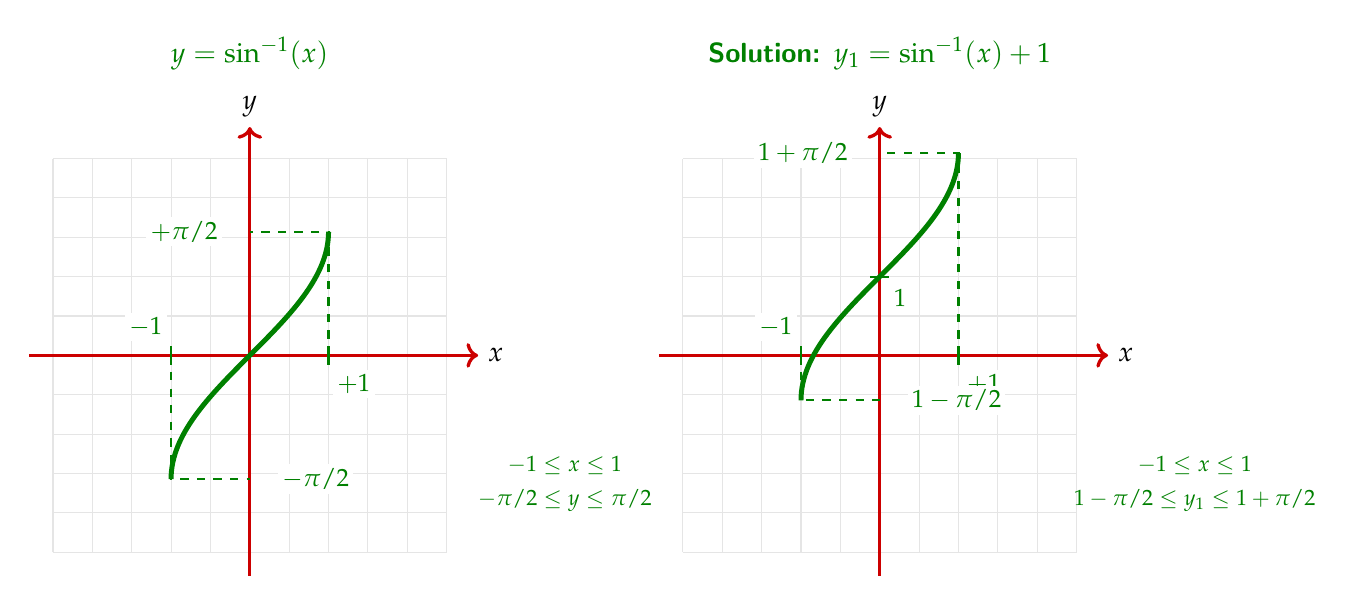
\begin{tikzpicture}[
    scale=1.0,
    axisline/.style={red!80!black, line width=1.2pt, ->},
    curve/.style={green!50!black, line width=1.8pt},
    guide/.style={green!50!black, thick, dashed},
    lbl/.style={green!50!black, font=\small\bfseries,
                fill=white, inner sep=1.5pt}
]

% =========================================================
% FIRST GRAPH: y = sin^{-1}(x)
% =========================================================
\draw[lightgray!40, thin, step=0.5] (-2.5,-2.5) grid (2.5,2.5);

\draw[axisline] (-2.8,0) -- (2.9,0) node[right, black, inner sep=3pt] {$x$};
\draw[axisline] (0,-2.8) -- (0,2.9) node[above, black, inner sep=3pt] {$y$};

% x-axis ticks
\draw[green!50!black, thick] (-1,-0.12) -- (-1,0.12);
\draw[green!50!black, thick] (1,-0.12) -- (1,0.12);
\node[lbl, anchor=south east] at (-1.05,0.18) {$-1$};
\node[lbl, anchor=north west] at (1.05,-0.18) {$+1$};

% dashed reference lines
\draw[guide] (-1,0) -- (-1,-1.5708) -- (0,-1.5708);
\draw[guide] (1,0) -- (1,1.5708) -- (0,1.5708);

% y-axis labels, pushed off the axis
\node[lbl, anchor=east] at (-0.35,1.5708) {$+\pi/2$};
\node[lbl, anchor=west] at (0.35,-1.5708) {$-\pi/2$};

% curve
\draw[curve, smooth] plot[domain=-1.5708:1.5708, samples=60] ({sin(\x r)}, \x);

% title above the grid
\node[green!50!black, font=\bfseries, anchor=south] at (0,3.5)
      {$y = \sin^{-1}(x)$};

% domain and range below the grid
\node[green!50!black, font=\footnotesize\bfseries, align=center, anchor=north]
      at (4,-1.15) { $-1 \le x \le 1$ \\[3pt] $-\pi/2 \le y \le \pi/2$};

% =========================================================
% SECOND GRAPH: empty grid
% =========================================================
\begin{scope}[shift={(8,0)}]
  \draw[lightgray!40, thin, step=0.5] (-2.5,-2.5) grid (2.5,2.5);
  \draw[axisline] (-2.8,0) -- (2.9,0) node[right, black, inner sep=3pt] {$x$};
  \draw[axisline] (0,-2.8) -- (0,2.9) node[above, black, inner sep=3pt] {$y$};
  
    % x-axis ticks
  \draw[green!50!black, thick] (-1,-0.12) -- (-1,0.12);
  \draw[green!50!black, thick] (1,-0.12) -- (1,0.12);
  \node[lbl, anchor=south east] at (-1.05,0.18) {$-1$};
  \node[lbl, anchor=north west] at (1.05,-0.18) {$+1$};

  % y-intercept tick at (0,1)
  \draw[green!50!black, thick] (-0.12,1) -- (0.12,1);
  \node[lbl, anchor=north west] at (0.12,0.9) {$1$};

  % dashed reference lines to the shifted endpoints
  \draw[guide] (-1,0) -- (-1,-0.5708) -- (0,-0.5708);
  \draw[guide] (1,0) -- (1,2.5708) -- (0,2.5708);

  % y-axis labels, pushed off the axis
  \node[lbl, anchor=east] at (-0.35,2.5708) {$1+\pi/2$};
  \node[lbl, anchor=west] at (0.35,-0.5708) {$1-\pi/2$};

  % curve: same parametrisation, shifted up by 1
  \draw[curve, smooth] plot[domain=-1.5708:1.5708, samples=60] ({sin(\x r)}, {\x+1});

  % title above the grid
  \node[green!50!black, font=\bfseries, anchor=south] at (0,3.5)
        {Solution: $y_1 = \sin^{-1}(x) + 1$};

  % domain and range beside the grid
  \node[green!50!black, font=\footnotesize\bfseries, align=center, anchor=north]
        at (4,-1.15) {$-1 \le x \le 1$ \\[3pt] $1-\pi/2 \le y_1 \le 1+\pi/2$};
        
\end{scope}

\end{tikzpicture}

\item Consider $y = \sin(x)$. Based on this, plot $y_1 = \frac{1}{2}\sin(x)$.  \hfill \textbf{(2.5 Points)}

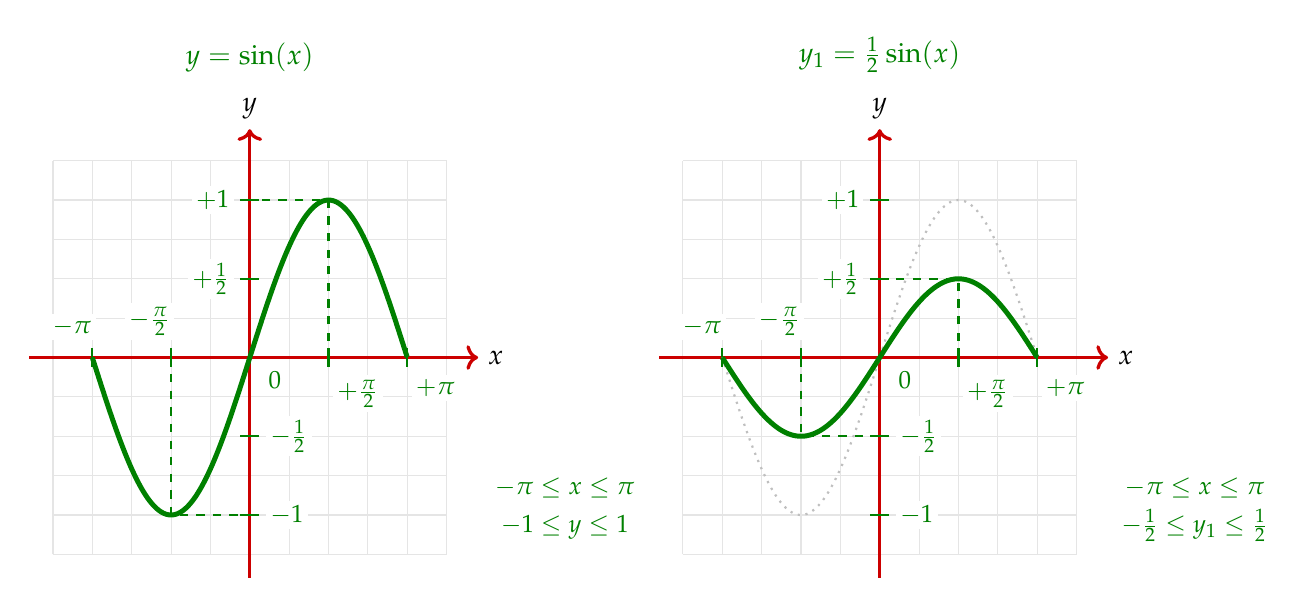
\begin{tikzpicture}[
    scale=1.0,
    axisline/.style={red!80!black, line width=1.2pt, ->},
    curve/.style={green!50!black, line width=1.8pt},
    guide/.style={green!50!black, thick, dashed},
    lbl/.style={green!50!black, font=\small\bfseries,
                fill=white, inner sep=1.5pt},
    % --- one panel: grid, axes, ticks and tick labels ---
    % One horizontal grid unit is pi/2 in x.
    % One vertical grid unit is 1/2 in y.
    pics/panel/.style={code={
        \draw[lightgray!40, thin, step=0.5] (-2.5,-2.5) grid (2.5,2.5);
        \draw[axisline] (-2.8,0) -- (2.9,0) node[right, black, inner sep=3pt] {$x$};
        \draw[axisline] (0,-2.8) -- (0,2.9) node[above, black, inner sep=3pt] {$y$};
        % x-axis ticks at -pi, -pi/2, pi/2, pi
        \foreach \u in {-2,-1,1,2}
          \draw[green!50!black, thick] (\u,-0.12) -- (\u,0.12);
        \node[lbl, anchor=south east] at (-0.95,0.22) {$-\tfrac{\pi}{2}$};
        \node[lbl, anchor=south east] at (-1.95,0.22) {$-\pi$};
        \node[lbl, anchor=north west] at (1.05,-0.22) {$+\tfrac{\pi}{2}$};
        \node[lbl, anchor=north west] at (2.05,-0.22) {$+\pi$};
        % y-axis ticks at -1, -1/2, 1/2, 1
        \foreach \v in {-2,-1,1,2}
          \draw[green!50!black, thick] (-0.12,\v) -- (0.12,\v);
        \node[lbl, anchor=east] at (-0.2,2) {$+1$};
        \node[lbl, anchor=east] at (-0.2,1) {$+\tfrac{1}{2}$};
        \node[lbl, anchor=west] at (0.2,-1) {$-\tfrac{1}{2}$};
        \node[lbl, anchor=west] at (0.2,-2) {$-1$};
%        \node[lbl, anchor=south west] at (0.18,0.12) {$0$};
        \node[lbl, anchor=north west] at (0.18,-0.12) {$0$};
    }}
]

% =========================================================
% FIRST PANEL: y = sin(x)
% =========================================================
\pic at (0,0) {panel};

% dashed reference lines to the peak and the trough
\draw[guide] (1,0) -- (1,2) -- (0,2);
\draw[guide] (-1,0) -- (-1,-2) -- (0,-2);

\draw[curve, smooth] plot[domain=-2:2, samples=120] (\x, {2*sin(\x*90)});

\node[green!50!black, font=\bfseries, anchor=south] at (0,3.5) {$y = \sin(x)$};

\node[green!50!black, font=\small\bfseries, align=center, anchor=north]
      at (4,-1.4) {$-\pi \le x \le \pi$ \\[3pt] $-1 \le y \le 1$};

% =========================================================
% SECOND PANEL: same grid and ticks, no curve
% =========================================================
\pic at (8,0) {panel};
\begin{scope}[shift={(8,0)}]
  % dashed reference lines to the new peak and trough
  \draw[guide] (1,0) -- (1,1) -- (0,1);
  \draw[guide] (-1,0) -- (-1,-1) -- (0,-1);

  % optional: the original y = sin(x), faint, for comparison
  \draw[gray!50, thick, dotted, smooth] plot[domain=-2:2, samples=120] (\x, {2*sin(\x*90)});

  % y1 = (1/2) sin(x): canvas height is half that of the first panel
  \draw[curve, smooth] plot[domain=-2:2, samples=120] (\x, {sin(\x*90)});

  \node[green!50!black, font=\bfseries, anchor=south] at (0,3.5)
        {$y_1 = \tfrac{1}{2}\sin(x)$};

  \node[green!50!black, font=\small\bfseries, align=center, anchor=north]
        at (4,-1.4) {$-\pi \le x \le \pi$ \\[3pt] $-\tfrac{1}{2} \le y_1 \le \tfrac{1}{2}$};
\end{scope}


\end{tikzpicture}
\end{enumerate}


\end{document}